%%%%%%%%%%%%%%%%%%%%%%%%%%%%%%%%%%%%%%%%%%%%%%%%%%%%%%%%%%%%%%%%%%%%%%%%%%%%%%%
%% SelfHealingNN: Project Implementation Guide
%% A Blueprint for AI and Human Implementers
%%%%%%%%%%%%%%%%%%%%%%%%%%%%%%%%%%%%%%%%%%%%%%%%%%%%%%%%%%%%%%%%%%%%%%%%%%%%%%%

\documentclass[11pt,a4paper]{article}

\usepackage[margin=1in]{geometry}
\usepackage{tikz}
\usepackage{booktabs}
\usepackage{tabularx}
\usepackage{xcolor}
\usepackage{hyperref}
\usepackage{enumitem}
\usepackage{fancyhdr}
\usepackage{tcolorbox}
\usepackage{forest}

\usetikzlibrary{shapes.geometric,arrows.meta,positioning,fit,calc,shadows,backgrounds}

%% Colors
\definecolor{encoderblue}{RGB}{52,152,219}
\definecolor{decodergreen}{RGB}{46,204,113}
\definecolor{classifierorange}{RGB}{230,126,34}
\definecolor{noisered}{RGB}{231,76,60}
\definecolor{stepcolor}{RGB}{41,128,185}
\definecolor{filecolor}{RGB}{155,89,182}

%% Box styles
\newtcolorbox{conceptbox}[1]{
    colback=stepcolor!10,
    colframe=stepcolor,
    fonttitle=\bfseries,
    title=#1,
    rounded corners,
    boxrule=1pt
}

\newtcolorbox{filebox}[1]{
    colback=filecolor!10,
    colframe=filecolor,
    fonttitle=\bfseries\ttfamily,
    title=#1,
    rounded corners,
    boxrule=1pt
}

\newtcolorbox{taskbox}{
    colback=gray!10,
    colframe=gray!50,
    rounded corners,
    boxrule=0.5pt
}

\hypersetup{colorlinks=true, linkcolor=stepcolor, urlcolor=stepcolor}

\pagestyle{fancy}
\fancyhf{}
\fancyhead[L]{\small SelfHealingNN Implementation Guide}
\fancyhead[R]{\small\thepage}
\renewcommand{\headrulewidth}{0.4pt}

\begin{document}

%%%%%%%%%%%%%%%%%%%%%%%%%%%%%%%%%%%%%%%%%%%%%%%%%%%%%%%%%%%%%%%%%%%%%%%%%%%%%%%
%% TITLE PAGE
%%%%%%%%%%%%%%%%%%%%%%%%%%%%%%%%%%%%%%%%%%%%%%%%%%%%%%%%%%%%%%%%%%%%%%%%%%%%%%%

\begin{center}
    {\Huge\bfseries SelfHealingNN}\\[0.3cm]
    {\LARGE Implementation Blueprint}\\[0.5cm]
    {\large A Step-by-Step Guide for Building a\\Two-Stage Self-Healing Image Classification System}\\[1cm]

    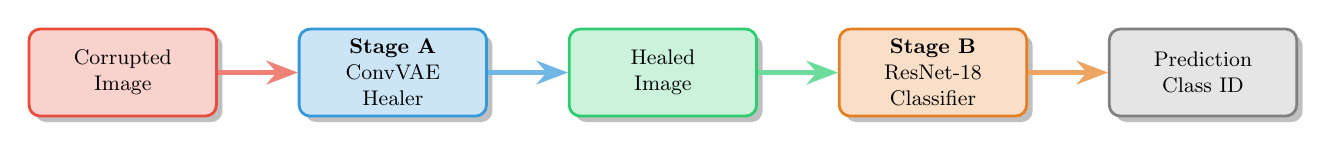
\begin{tikzpicture}[
        scale=0.85,
        transform shape,
        node distance=1.2cm,
        block/.style={draw, rounded corners, minimum width=2.8cm, minimum height=1.3cm, align=center, font=\small, drop shadow, line width=1pt},
        arrow/.style={-{Stealth[length=4mm]}, line width=2pt}
    ]
        \node[block, fill=noisered!25, draw=noisered] (noisy) {Corrupted\\Image};
        \node[block, fill=encoderblue!25, draw=encoderblue, right=of noisy] (vae) {\textbf{Stage A}\\ConvVAE\\Healer};
        \node[block, fill=decodergreen!25, draw=decodergreen, right=of vae] (healed) {Healed\\Image};
        \node[block, fill=classifierorange!25, draw=classifierorange, right=of healed] (resnet) {\textbf{Stage B}\\ResNet-18\\Classifier};
        \node[block, fill=gray!20, draw=gray, right=of resnet] (pred) {Prediction\\Class ID};

        \draw[arrow, noisered!70] (noisy) -- (vae);
        \draw[arrow, encoderblue!70] (vae) -- (healed);
        \draw[arrow, decodergreen!70] (healed) -- (resnet);
        \draw[arrow, classifierorange!70] (resnet) -- (pred);
    \end{tikzpicture}

    \vspace{0.8cm}
    {\large\textbf{Tech Stack:} PyTorch 2.x $\bullet$ ImageNet-100 $\bullet$ ResNet-18 $\bullet$ ConvVAE}
\end{center}

\vspace{0.5cm}

\begin{conceptbox}{What This Guide Is}
This document is an \textbf{implementation blueprint}---not a code tutorial. It describes:
\begin{itemize}[noitemsep]
    \item The purpose and responsibility of each file
    \item What components/functions each file should contain
    \item How files interact with each other
    \item Step-by-step build order
    \item Expected inputs, outputs, and behaviors
\end{itemize}
\textbf{For AI models:} Use this as a specification to generate the implementation.\\
\textbf{For humans:} Use this as a roadmap to understand what to build.
\end{conceptbox}

\tableofcontents
\newpage

%%%%%%%%%%%%%%%%%%%%%%%%%%%%%%%%%%%%%%%%%%%%%%%%%%%%%%%%%%%%%%%%%%%%%%%%%%%%%%%
%% SECTION 1: PROJECT OVERVIEW
%%%%%%%%%%%%%%%%%%%%%%%%%%%%%%%%%%%%%%%%%%%%%%%%%%%%%%%%%%%%%%%%%%%%%%%%%%%%%%%

\section{Project Overview}

\subsection{Problem Statement}
Neural network classifiers trained on clean images suffer severe accuracy degradation when inputs are corrupted by noise (Gaussian noise, salt-and-pepper noise, occlusions, etc.). This project builds a two-stage ``self-healing'' pipeline that:
\begin{enumerate}[noitemsep]
    \item \textbf{Stage A (Healer):} A Convolutional VAE reconstructs clean images from corrupted inputs
    \item \textbf{Stage B (Classifier):} A pretrained ResNet-18 classifies the healed images
\end{enumerate}

\subsection{Expected Results}
\begin{center}
\begin{tabular}{@{}lcc@{}}
\toprule
\textbf{Pipeline} & \textbf{Accuracy} & \textbf{Notes} \\
\midrule
Clean $\rightarrow$ Classifier & $\sim$94\% & Baseline \\
Noisy $\rightarrow$ Classifier & $\sim$52\% & Degraded \\
Noisy $\rightarrow$ VAE $\rightarrow$ Classifier & $\sim$88\% & Recovered \\
\bottomrule
\end{tabular}
\end{center}

\subsection{Dataset}
\begin{itemize}[noitemsep]
    \item \textbf{Name:} ImageNet-100 (subset of ImageNet with 100 classes)
    \item \textbf{Source:} Kaggle (\texttt{ambityga/imagenet100})
    \item \textbf{Structure:} Folder per class, JPEG images
    \item \textbf{Image size:} 224$\times$224$\times$3 (resized)
    \item \textbf{Split:} 80\% train, 10\% validation, 10\% test
\end{itemize}

\newpage

%%%%%%%%%%%%%%%%%%%%%%%%%%%%%%%%%%%%%%%%%%%%%%%%%%%%%%%%%%%%%%%%%%%%%%%%%%%%%%%
%% SECTION 2: ARCHITECTURE
%%%%%%%%%%%%%%%%%%%%%%%%%%%%%%%%%%%%%%%%%%%%%%%%%%%%%%%%%%%%%%%%%%%%%%%%%%%%%%%

\section{System Architecture}

\subsection{Pipeline Flow}

\begin{center}
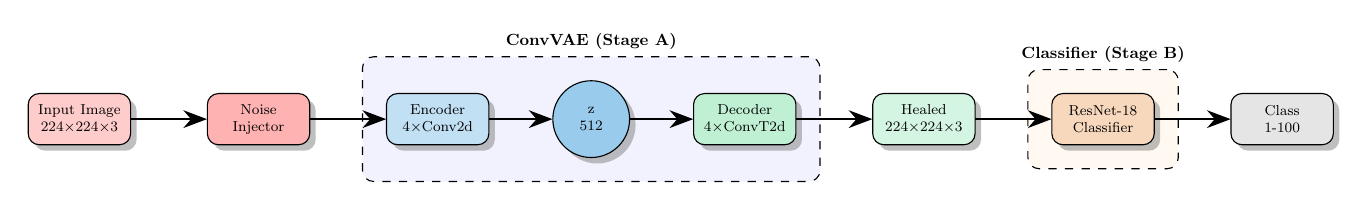
\begin{tikzpicture}[
    scale=0.65,
    transform shape,
    block/.style={draw, rounded corners, minimum width=2cm, minimum height=1cm, align=center, font=\footnotesize, drop shadow},
    arrow/.style={-{Stealth[length=3mm]}, thick}
]
    \node[block, fill=red!20] (input) at (0,0) {Input Image\\224$\times$224$\times$3};
    \node[block, fill=red!30] (noise) at (3.5,0) {Noise\\Injector};
    \node[block, fill=encoderblue!30] (enc) at (7,0) {Encoder\\4$\times$Conv2d};
    \node[block, fill=encoderblue!50, circle, minimum width=1.5cm] (latent) at (10,0) {z\\512};
    \node[block, fill=decodergreen!30] (dec) at (13,0) {Decoder\\4$\times$ConvT2d};
    \node[block, fill=decodergreen!20] (healed) at (16.5,0) {Healed\\224$\times$224$\times$3};
    \node[block, fill=classifierorange!30] (classifier) at (20,0) {ResNet-18\\Classifier};
    \node[block, fill=gray!20] (output) at (23.5,0) {Class\\1-100};

    \draw[arrow] (input) -- (noise);
    \draw[arrow] (noise) -- (enc);
    \draw[arrow] (enc) -- (latent);
    \draw[arrow] (latent) -- (dec);
    \draw[arrow] (dec) -- (healed);
    \draw[arrow] (healed) -- (classifier);
    \draw[arrow] (classifier) -- (output);

    \begin{scope}[on background layer]
        \node[draw, dashed, rounded corners, fill=blue!5, fit=(enc)(latent)(dec), inner sep=0.3cm, label={[font=\small\bfseries]above:ConvVAE (Stage A)}] {};
        \node[draw, dashed, rounded corners, fill=orange!5, fit=(classifier), inner sep=0.3cm, label={[font=\small\bfseries]above:Classifier (Stage B)}] {};
    \end{scope}
\end{tikzpicture}
\end{center}

\subsection{ConvVAE Architecture}

\begin{center}
\begin{tabular}{@{}llll@{}}
\toprule
\textbf{Component} & \textbf{Layers} & \textbf{Channel Progression} & \textbf{Spatial Size} \\
\midrule
Input & --- & 3 & 224$\times$224 \\
Encoder Block 1 & Conv2d + BN + LeakyReLU & 3 $\rightarrow$ 64 & 224 $\rightarrow$ 112 \\
Encoder Block 2 & Conv2d + BN + LeakyReLU & 64 $\rightarrow$ 128 & 112 $\rightarrow$ 56 \\
Encoder Block 3 & Conv2d + BN + LeakyReLU & 128 $\rightarrow$ 256 & 56 $\rightarrow$ 28 \\
Encoder Block 4 & Conv2d + BN + LeakyReLU & 256 $\rightarrow$ 512 & 28 $\rightarrow$ 14 \\
\midrule
Flatten + FC & Linear & 512$\times$14$\times$14 $\rightarrow$ 512 & --- \\
Latent & $\mu$, $\log\sigma^2$ & 512 (each) & --- \\
\midrule
FC + Reshape & Linear & 512 $\rightarrow$ 512$\times$14$\times$14 & 14$\times$14 \\
Decoder Block 1 & ConvT2d + BN + LeakyReLU & 512 $\rightarrow$ 256 & 14 $\rightarrow$ 28 \\
Decoder Block 2 & ConvT2d + BN + LeakyReLU & 256 $\rightarrow$ 128 & 28 $\rightarrow$ 56 \\
Decoder Block 3 & ConvT2d + BN + LeakyReLU & 128 $\rightarrow$ 64 & 56 $\rightarrow$ 112 \\
Decoder Block 4 & ConvT2d + Sigmoid & 64 $\rightarrow$ 3 & 112 $\rightarrow$ 224 \\
\bottomrule
\end{tabular}
\end{center}

\textbf{Conv2d parameters:} kernel\_size=4, stride=2, padding=1 (halves spatial dimensions)\\
\textbf{ConvTranspose2d parameters:} kernel\_size=4, stride=2, padding=1 (doubles spatial dimensions)

\subsection{Classifier Architecture}
\begin{itemize}[noitemsep]
    \item Use pretrained ResNet-18 from torchvision
    \item Replace final fully-connected layer: 512 $\rightarrow$ 100 (number of classes)
    \item Apply ImageNet normalization (mean=[0.485, 0.456, 0.406], std=[0.229, 0.224, 0.225])
\end{itemize}

\newpage

%%%%%%%%%%%%%%%%%%%%%%%%%%%%%%%%%%%%%%%%%%%%%%%%%%%%%%%%%%%%%%%%%%%%%%%%%%%%%%%
%% SECTION 3: FILE STRUCTURE
%%%%%%%%%%%%%%%%%%%%%%%%%%%%%%%%%%%%%%%%%%%%%%%%%%%%%%%%%%%%%%%%%%%%%%%%%%%%%%%

\section{Project File Structure}

\begin{center}
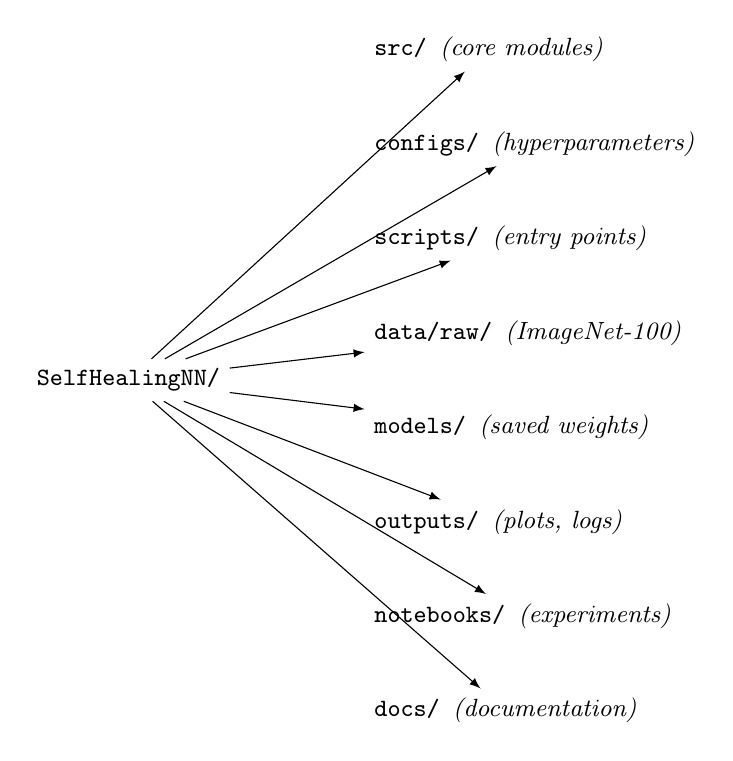
\begin{tikzpicture}[
    grow'=right,
    level distance=3cm,
    sibling distance=0.4cm,
    edge from parent/.style={draw, -latex},
    every node/.style={font=\ttfamily\small, anchor=west},
    level 1/.style={sibling distance=1.2cm},
]
\node {SelfHealingNN/}
    child { node {\textbf{src/} \textnormal{\textit{(core modules)}}}}
    child { node {\textbf{configs/} \textnormal{\textit{(hyperparameters)}}}}
    child { node {\textbf{scripts/} \textnormal{\textit{(entry points)}}}}
    child { node {\textbf{data/raw/} \textnormal{\textit{(ImageNet-100)}}}}
    child { node {\textbf{models/} \textnormal{\textit{(saved weights)}}}}
    child { node {\textbf{outputs/} \textnormal{\textit{(plots, logs)}}}}
    child { node {\textbf{notebooks/} \textnormal{\textit{(experiments)}}}}
    child { node {\textbf{docs/} \textnormal{\textit{(documentation)}}}};
\end{tikzpicture}
\end{center}

\subsection{Complete File List}

\begin{center}
\begin{tabular}{@{}lll@{}}
\toprule
\textbf{File Path} & \textbf{Purpose} & \textbf{Build Order} \\
\midrule
\texttt{configs/config.yaml} & All hyperparameters & 1 \\
\texttt{src/\_\_init\_\_.py} & Package marker (empty) & 2 \\
\texttt{src/dataset.py} & Data loading \& noise injection & 3 \\
\texttt{src/conv\_vae.py} & VAE model definition & 4 \\
\texttt{src/classifier.py} & ResNet-18 classifier & 5 \\
\texttt{src/train\_vae.py} & VAE training logic & 6 \\
\texttt{src/train\_classifier.py} & Classifier training logic & 7 \\
\texttt{src/pipeline.py} & End-to-end inference & 8 \\
\texttt{src/evaluate.py} & Evaluation metrics & 9 \\
\texttt{scripts/train\_vae\_runner.py} & CLI to train VAE & 10 \\
\texttt{scripts/train\_classifier\_runner.py} & CLI to train classifier & 11 \\
\texttt{scripts/evaluate\_runner.py} & CLI to run evaluation & 12 \\
\bottomrule
\end{tabular}
\end{center}

\newpage

%%%%%%%%%%%%%%%%%%%%%%%%%%%%%%%%%%%%%%%%%%%%%%%%%%%%%%%%%%%%%%%%%%%%%%%%%%%%%%%
%% SECTION 4: FILE SPECIFICATIONS
%%%%%%%%%%%%%%%%%%%%%%%%%%%%%%%%%%%%%%%%%%%%%%%%%%%%%%%%%%%%%%%%%%%%%%%%%%%%%%%

\section{File Specifications}

%% CONFIG %%
\begin{filebox}{configs/config.yaml}
\textbf{Purpose:} Central configuration file for all hyperparameters.

\textbf{Sections to include:}
\begin{itemize}[noitemsep]
    \item \texttt{dataset:} root path, image\_size (224), num\_classes (100), train\_split (0.8)
    \item \texttt{noise:} types list, gaussian\_std (0.3), salt\_pepper\_prob (0.1), occlusion\_size (32)
    \item \texttt{vae:} latent\_dim (512), encoder\_channels [64,128,256,512], beta (0.5), learning\_rate (3e-4), epochs (50), batch\_size (32)
    \item \texttt{classifier:} backbone (resnet18), pretrained (true), learning\_rate (1e-4), epochs (30), batch\_size (32)
    \item \texttt{training:} device (cuda), num\_workers (4), early\_stopping\_patience (7)
\end{itemize}
\end{filebox}

\vspace{0.5cm}

%% DATASET %%
\begin{filebox}{src/dataset.py}
\textbf{Purpose:} Data loading, preprocessing, and noise injection.

\textbf{Components to implement:}
\begin{enumerate}[noitemsep]
    \item \textbf{Constants:} ImageNet mean [0.485, 0.456, 0.406] and std [0.229, 0.224, 0.225]
    \item \textbf{Class NoiseInjector:} Methods for adding noise to tensors
    \begin{itemize}[noitemsep]
        \item \texttt{add\_gaussian\_noise(image, std)} --- add Gaussian noise, clamp to valid range
        \item \texttt{add\_salt\_pepper(image, prob)} --- randomly set pixels to min/max values
        \item \texttt{add\_occlusion(image, patch\_size)} --- black out random rectangular patch
    \end{itemize}
    \item \textbf{Class ImageNet100Dataset:} Wraps torchvision.datasets.ImageFolder
    \begin{itemize}[noitemsep]
        \item Transform pipeline: Resize $\rightarrow$ CenterCrop $\rightarrow$ ToTensor $\rightarrow$ Normalize
        \item Returns (image, label) tuples
    \end{itemize}
    \item \textbf{Class NoisyImageNet100Dataset:} Wraps base dataset, adds noise
    \begin{itemize}[noitemsep]
        \item Constructor takes: base\_dataset, noise\_type, noise\_params, return\_clean flag
        \item Returns (noisy\_image, clean\_image, label) for VAE training
        \item Returns (noisy\_image, label) for classifier testing
    \end{itemize}
    \item \textbf{Function get\_dataloaders:} Factory function
    \begin{itemize}[noitemsep]
        \item Splits dataset into train/val/test (80/10/10)
        \item Returns three DataLoader objects
        \item Accepts flags for noisy mode and noise parameters
    \end{itemize}
\end{enumerate}
\end{filebox}

\newpage

%% CONV_VAE %%
\begin{filebox}{src/conv\_vae.py}
\textbf{Purpose:} Convolutional Variational Autoencoder model.

\textbf{Components to implement:}
\begin{enumerate}[noitemsep]
    \item \textbf{Class ConvEncoder:}
    \begin{itemize}[noitemsep]
        \item 4 convolutional blocks (Conv2d + BatchNorm + LeakyReLU)
        \item Channel progression: 3 $\rightarrow$ 64 $\rightarrow$ 128 $\rightarrow$ 256 $\rightarrow$ 512
        \item Flatten output and project to $\mu$ and $\log\sigma^2$ vectors (latent\_dim each)
        \item Forward returns: (mu, logvar)
    \end{itemize}
    \item \textbf{Class ConvDecoder:}
    \begin{itemize}[noitemsep]
        \item FC layer from latent\_dim to 512$\times$14$\times$14
        \item 4 transposed conv blocks (ConvTranspose2d + BatchNorm + LeakyReLU)
        \item Final layer uses Sigmoid activation (output in [0,1])
        \item Forward returns: reconstructed image
    \end{itemize}
    \item \textbf{Class ConvVAE:}
    \begin{itemize}[noitemsep]
        \item Contains encoder and decoder
        \item Implements reparameterization trick: $z = \mu + \sigma \cdot \epsilon$
        \item Forward returns: (reconstruction, mu, logvar)
    \end{itemize}
    \item \textbf{Function vae\_loss:}
    \begin{itemize}[noitemsep]
        \item MSE reconstruction loss between output and target
        \item KL divergence: $-0.5 \times \text{mean}(1 + \log\sigma^2 - \mu^2 - \sigma^2)$
        \item Total loss = recon\_loss + $\beta$ $\times$ kl\_loss
        \item Returns: (total\_loss, dict with component losses)
    \end{itemize}
\end{enumerate}
\end{filebox}

\vspace{0.5cm}

%% CLASSIFIER %%
\begin{filebox}{src/classifier.py}
\textbf{Purpose:} Image classifier using pretrained ResNet-18.

\textbf{Components to implement:}
\begin{enumerate}[noitemsep]
    \item \textbf{Class SelfHealingClassifier:}
    \begin{itemize}[noitemsep]
        \item Load ResNet-18 with ImageNet pretrained weights
        \item Replace final FC layer: 512 $\rightarrow$ num\_classes (100)
        \item Forward returns: logits (before softmax)
    \end{itemize}
    \item \textbf{Function get\_classifier:} Factory function with num\_classes and pretrained args
\end{enumerate}
\end{filebox}

\newpage

%% TRAIN_VAE %%
\begin{filebox}{src/train\_vae.py}
\textbf{Purpose:} Training loop for the VAE.

\textbf{Components to implement:}
\begin{enumerate}[noitemsep]
    \item \textbf{Function train\_vae:}
    \begin{itemize}[noitemsep]
        \item Arguments: model, train\_loader, val\_loader, device, epochs, lr, beta, save\_path
        \item Optimizer: AdamW
        \item Scheduler: CosineAnnealingLR
        \item Training loop:
        \begin{itemize}[noitemsep]
            \item For each batch: get (noisy, clean, label)
            \item Forward pass: recon, mu, logvar = model(noisy)
            \item Compute loss against clean target
            \item Backward and step
        \end{itemize}
        \item Validation loop: compute average validation loss (no gradients)
        \item Save best model based on validation loss
        \item Return training history dictionary
    \end{itemize}
    \item \textbf{Optional - Class EarlyStopping:} Stop if val loss doesn't improve for N epochs
\end{enumerate}
\end{filebox}

\vspace{0.5cm}

%% TRAIN_CLASSIFIER %%
\begin{filebox}{src/train\_classifier.py}
\textbf{Purpose:} Training loop for the classifier.

\textbf{Components to implement:}
\begin{enumerate}[noitemsep]
    \item \textbf{Function train\_classifier:}
    \begin{itemize}[noitemsep]
        \item Arguments: model, train\_loader, val\_loader, device, epochs, lr, save\_path
        \item Loss function: CrossEntropyLoss
        \item Optimizer: AdamW
        \item \textbf{Two-phase training strategy:}
        \begin{itemize}[noitemsep]
            \item Phase 1 (5 epochs): Freeze all backbone layers, train only final FC
            \item Phase 2 (remaining epochs): Unfreeze all, fine-tune entire network with lower LR
        \end{itemize}
        \item Validation: compute accuracy
        \item Save best model based on validation accuracy
        \item Return training history dictionary
    \end{itemize}
\end{enumerate}
\end{filebox}

\newpage

%% PIPELINE %%
\begin{filebox}{src/pipeline.py}
\textbf{Purpose:} End-to-end inference combining VAE and classifier.

\textbf{Components to implement:}
\begin{enumerate}[noitemsep]
    \item \textbf{Class SelfHealingPipeline:}
    \begin{itemize}[noitemsep]
        \item Constructor takes: vae model, classifier model
        \item \texttt{heal(noisy\_image)} method: pass through VAE, return reconstruction
        \item \texttt{forward(noisy\_image)} method: heal then classify
        \begin{itemize}[noitemsep]
            \item Returns: (predicted\_class, confidence, healed\_image)
        \end{itemize}
        \item \texttt{save(path)} method: save both model state dicts to single file
        \item \texttt{load(path, device)} method: load state dicts into models
    \end{itemize}
    \item All inference methods should use \texttt{@torch.no\_grad()} decorator
\end{enumerate}
\end{filebox}

\vspace{0.5cm}

%% EVALUATE %%
\begin{filebox}{src/evaluate.py}
\textbf{Purpose:} Evaluation metrics and comparison functions.

\textbf{Components to implement:}
\begin{enumerate}[noitemsep]
    \item \textbf{Function evaluate\_classifier:}
    \begin{itemize}[noitemsep]
        \item Compute accuracy, top-5 accuracy, confusion matrix
        \item Arguments: model, dataloader, device
        \item Returns: dict with metrics
    \end{itemize}
    \item \textbf{Function evaluate\_pipeline:}
    \begin{itemize}[noitemsep]
        \item Run full pipeline (noisy $\rightarrow$ VAE $\rightarrow$ classifier)
        \item Compare against baseline (noisy $\rightarrow$ classifier only)
        \item Returns: dict with both accuracy sets
    \end{itemize}
    \item \textbf{Function compute\_reconstruction\_metrics:}
    \begin{itemize}[noitemsep]
        \item PSNR (Peak Signal-to-Noise Ratio)
        \item SSIM (Structural Similarity Index) - use scikit-image
        \item Arguments: original\_images, reconstructed\_images
    \end{itemize}
    \item \textbf{Function evaluate\_noise\_robustness:}
    \begin{itemize}[noitemsep]
        \item Test at multiple noise levels (0.1, 0.2, 0.3, 0.5, 0.7)
        \item Returns: table of accuracies per noise level
    \end{itemize}
\end{enumerate}
\end{filebox}

\newpage

%% RUNNER SCRIPTS %%
\begin{filebox}{scripts/train\_vae\_runner.py}
\textbf{Purpose:} Command-line entry point for VAE training.

\textbf{Implementation:}
\begin{enumerate}[noitemsep]
    \item Add parent directory to sys.path for imports
    \item Load config.yaml
    \item Create noisy dataloaders (return\_clean=True)
    \item Instantiate ConvVAE model
    \item Call train\_vae function
    \item Optionally save training plots to outputs/plots/
\end{enumerate}
\end{filebox}

\vspace{0.3cm}

\begin{filebox}{scripts/train\_classifier\_runner.py}
\textbf{Purpose:} Command-line entry point for classifier training.

\textbf{Implementation:}
\begin{enumerate}[noitemsep]
    \item Load config.yaml
    \item Create clean dataloaders (no noise)
    \item Instantiate SelfHealingClassifier
    \item Call train\_classifier function
    \item Save training plots
\end{enumerate}
\end{filebox}

\vspace{0.3cm}

\begin{filebox}{scripts/evaluate\_runner.py}
\textbf{Purpose:} Command-line entry point for evaluation.

\textbf{Implementation:}
\begin{enumerate}[noitemsep]
    \item Load trained VAE and classifier from models/ directory
    \item Create SelfHealingPipeline
    \item Run evaluate\_pipeline on test set
    \item Run evaluate\_noise\_robustness at multiple noise levels
    \item Print results table and save to outputs/
\end{enumerate}
\end{filebox}

\newpage

%%%%%%%%%%%%%%%%%%%%%%%%%%%%%%%%%%%%%%%%%%%%%%%%%%%%%%%%%%%%%%%%%%%%%%%%%%%%%%%
%% SECTION 5: BUILD STEPS
%%%%%%%%%%%%%%%%%%%%%%%%%%%%%%%%%%%%%%%%%%%%%%%%%%%%%%%%%%%%%%%%%%%%%%%%%%%%%%%

\section{Step-by-Step Build Instructions}

\begin{conceptbox}{Phase 1: Environment Setup}
\begin{enumerate}[noitemsep]
    \item Create project directory structure as shown in Section 3
    \item Create Python virtual environment
    \item Install dependencies: torch, torchvision, numpy, matplotlib, scikit-image, scikit-learn, pyyaml, tqdm, pandas
    \item Verify CUDA availability
    \item Create \texttt{configs/config.yaml} with all parameters
\end{enumerate}
\end{conceptbox}

\vspace{0.3cm}

\begin{conceptbox}{Phase 2: Dataset Setup}
\begin{enumerate}[noitemsep]
    \item Download ImageNet-100 from Kaggle
    \item Extract to \texttt{data/raw/train/} (should have 100 subdirectories)
    \item Verify structure: each class folder contains JPEG images
    \item Implement \texttt{src/dataset.py}
    \item Test: create dataloaders, visualize a few samples with noise
\end{enumerate}
\end{conceptbox}

\vspace{0.3cm}

\begin{conceptbox}{Phase 3: Model Implementation}
\begin{enumerate}[noitemsep]
    \item Implement \texttt{src/conv\_vae.py}
    \begin{itemize}[noitemsep]
        \item Test: create model, pass random tensor, verify output shapes
        \item Encoder output: (batch, 512), (batch, 512) for mu/logvar
        \item Decoder output: (batch, 3, 224, 224)
    \end{itemize}
    \item Implement \texttt{src/classifier.py}
    \begin{itemize}[noitemsep]
        \item Test: verify ResNet loads, final layer outputs 100 classes
    \end{itemize}
    \item Implement \texttt{src/pipeline.py}
    \begin{itemize}[noitemsep]
        \item Test: combine untrained models, verify forward pass works
    \end{itemize}
\end{enumerate}
\end{conceptbox}

\vspace{0.3cm}

\begin{conceptbox}{Phase 4: Training Implementation}
\begin{enumerate}[noitemsep]
    \item Implement \texttt{src/train\_vae.py}
    \item Implement \texttt{src/train\_classifier.py}
    \item Create runner scripts in \texttt{scripts/}
    \item Test with 1-2 epochs to verify everything works
\end{enumerate}
\end{conceptbox}

\newpage

\begin{conceptbox}{Phase 5: Full Training}
\begin{enumerate}[noitemsep]
    \item \textbf{Train VAE first:}
    \begin{itemize}[noitemsep]
        \item Run: \texttt{python scripts/train\_vae\_runner.py}
        \item Expected time: $\sim$4-6 hours on RTX 3050
        \item Output: \texttt{models/conv\_vae\_best.pth} ($\sim$200 MB)
        \item Monitor: validation loss should decrease steadily
    \end{itemize}
    \item \textbf{Train classifier second:}
    \begin{itemize}[noitemsep]
        \item Run: \texttt{python scripts/train\_classifier\_runner.py}
        \item Expected time: $\sim$2-3 hours on RTX 3050
        \item Output: \texttt{models/resnet\_classifier.pth} ($\sim$45 MB)
        \item Monitor: validation accuracy should reach $\sim$90\%+
    \end{itemize}
\end{enumerate}
\end{conceptbox}

\vspace{0.3cm}

\begin{conceptbox}{Phase 6: Evaluation}
\begin{enumerate}[noitemsep]
    \item Implement \texttt{src/evaluate.py}
    \item Create \texttt{scripts/evaluate\_runner.py}
    \item Run evaluation: \texttt{python scripts/evaluate\_runner.py}
    \item Generate comparison table across noise levels
    \item Visualize: noisy $\rightarrow$ healed $\rightarrow$ prediction examples
\end{enumerate}
\end{conceptbox}

\newpage

%%%%%%%%%%%%%%%%%%%%%%%%%%%%%%%%%%%%%%%%%%%%%%%%%%%%%%%%%%%%%%%%%%%%%%%%%%%%%%%
%% SECTION 6: TRAINING DETAILS
%%%%%%%%%%%%%%%%%%%%%%%%%%%%%%%%%%%%%%%%%%%%%%%%%%%%%%%%%%%%%%%%%%%%%%%%%%%%%%%

\section{Training Details}

\subsection{VAE Training}

\begin{taskbox}
\textbf{Input:} Noisy image (corrupted)\\
\textbf{Target:} Clean image (original)\\
\textbf{Loss:} MSE(reconstruction, clean) + $\beta \times$ KL\_divergence\\
\textbf{Key insight:} VAE learns to remove noise by reconstructing the clean version
\end{taskbox}

\begin{center}
\begin{tabular}{@{}ll@{}}
\toprule
\textbf{Hyperparameter} & \textbf{Value} \\
\midrule
Optimizer & AdamW \\
Learning rate & 3e-4 \\
Scheduler & CosineAnnealingLR \\
Batch size & 32 \\
Epochs & 50 \\
$\beta$ (KL weight) & 0.5 \\
Latent dimension & 512 \\
\bottomrule
\end{tabular}
\end{center}

\subsection{Classifier Training}

\begin{taskbox}
\textbf{Input:} Clean image\\
\textbf{Target:} Class label (0-99)\\
\textbf{Loss:} CrossEntropyLoss\\
\textbf{Key insight:} Train on clean images; during inference, VAE provides ``clean-like'' inputs
\end{taskbox}

\begin{center}
\begin{tabular}{@{}ll@{}}
\toprule
\textbf{Hyperparameter} & \textbf{Value} \\
\midrule
Pretrained weights & ImageNet \\
Phase 1 (freeze backbone) & 5 epochs \\
Phase 2 (fine-tune all) & 25 epochs \\
Learning rate & 1e-4 \\
Batch size & 32 \\
\bottomrule
\end{tabular}
\end{center}

\newpage

%%%%%%%%%%%%%%%%%%%%%%%%%%%%%%%%%%%%%%%%%%%%%%%%%%%%%%%%%%%%%%%%%%%%%%%%%%%%%%%
%% SECTION 7: EXPECTED OUTPUTS
%%%%%%%%%%%%%%%%%%%%%%%%%%%%%%%%%%%%%%%%%%%%%%%%%%%%%%%%%%%%%%%%%%%%%%%%%%%%%%%

\section{Expected Outputs}

\subsection{Model Files}
\begin{center}
\begin{tabular}{@{}lll@{}}
\toprule
\textbf{File} & \textbf{Size} & \textbf{Contents} \\
\midrule
\texttt{models/conv\_vae\_best.pth} & $\sim$200 MB & VAE encoder + decoder weights \\
\texttt{models/resnet\_classifier.pth} & $\sim$45 MB & Fine-tuned ResNet-18 weights \\
\bottomrule
\end{tabular}
\end{center}

\subsection{Training Metrics}
\begin{itemize}[noitemsep]
    \item VAE: final validation loss $\sim$0.02--0.03
    \item Classifier: final validation accuracy $\sim$92--95\%
\end{itemize}

\subsection{Evaluation Metrics}
\begin{center}
\begin{tabular}{@{}lccc@{}}
\toprule
\textbf{Noise Level ($\sigma$)} & \textbf{Noisy$\rightarrow$Classifier} & \textbf{Noisy$\rightarrow$VAE$\rightarrow$Classifier} & \textbf{Recovery} \\
\midrule
0.1 & $\sim$82\% & $\sim$93\% & +11\% \\
0.2 & $\sim$68\% & $\sim$91\% & +23\% \\
0.3 & $\sim$52\% & $\sim$88\% & +36\% \\
0.5 & $\sim$32\% & $\sim$78\% & +46\% \\
0.7 & $\sim$19\% & $\sim$64\% & +45\% \\
\bottomrule
\end{tabular}
\end{center}

\subsection{Visualization Outputs}
\begin{itemize}[noitemsep]
    \item \texttt{outputs/plots/vae\_loss\_curve.png} --- training/validation loss over epochs
    \item \texttt{outputs/plots/classifier\_accuracy.png} --- accuracy over epochs
    \item \texttt{outputs/plots/reconstruction\_samples.png} --- noisy vs. healed comparisons
    \item \texttt{outputs/plots/noise\_robustness.png} --- accuracy vs. noise level graph
\end{itemize}

\newpage

%%%%%%%%%%%%%%%%%%%%%%%%%%%%%%%%%%%%%%%%%%%%%%%%%%%%%%%%%%%%%%%%%%%%%%%%%%%%%%%
%% SECTION 8: KEY IMPLEMENTATION NOTES
%%%%%%%%%%%%%%%%%%%%%%%%%%%%%%%%%%%%%%%%%%%%%%%%%%%%%%%%%%%%%%%%%%%%%%%%%%%%%%%

\section{Key Implementation Notes}

\begin{conceptbox}{Critical Details}
\begin{enumerate}
    \item \textbf{Normalization consistency:} Always apply ImageNet normalization (mean/std) to images. Both VAE and classifier must use the same normalization.

    \item \textbf{Noise clamping:} After adding noise, clamp values to valid range (approximately -3 to +3 for normalized images) to prevent extreme outliers.

    \item \textbf{VAE output activation:} Use Sigmoid on decoder output, then denormalize, or match the input range. Ensure reconstruction target matches output range.

    \item \textbf{Random seed:} Set seed for dataset splitting (42) to ensure reproducible train/val/test splits.

    \item \textbf{Two-phase classifier training:} Freezing the backbone initially prevents catastrophic forgetting of pretrained features.

    \item \textbf{Model saving:} Save state\_dict (not entire model) for compatibility.

    \item \textbf{Inference mode:} Use \texttt{model.eval()} and \texttt{torch.no\_grad()} during evaluation.

    \item \textbf{Device handling:} Move both model and data to same device (cuda/cpu).
\end{enumerate}
\end{conceptbox}

\vspace{0.5cm}

\begin{conceptbox}{Common Pitfalls to Avoid}
\begin{itemize}
    \item Not matching normalization between training and inference
    \item Forgetting to call \texttt{model.eval()} during validation
    \item Training VAE on clean$\rightarrow$clean instead of noisy$\rightarrow$clean
    \item Using reconstruction loss against noisy target (should be clean)
    \item Not unfreezing classifier backbone in phase 2
    \item Memory issues: reduce batch size if OOM
\end{itemize}
\end{conceptbox}

\newpage

%%%%%%%%%%%%%%%%%%%%%%%%%%%%%%%%%%%%%%%%%%%%%%%%%%%%%%%%%%%%%%%%%%%%%%%%%%%%%%%
%% SECTION 9: QUICK REFERENCE
%%%%%%%%%%%%%%%%%%%%%%%%%%%%%%%%%%%%%%%%%%%%%%%%%%%%%%%%%%%%%%%%%%%%%%%%%%%%%%%

\section{Quick Reference}

\subsection{Dependencies}
\begin{center}
\begin{tabular}{@{}ll@{}}
\toprule
\textbf{Package} & \textbf{Purpose} \\
\midrule
torch, torchvision & Deep learning framework \\
numpy & Numerical operations \\
matplotlib & Plotting \\
scikit-image & SSIM metric \\
scikit-learn & Train/test split utilities \\
pyyaml & Config file parsing \\
tqdm & Progress bars \\
pandas & Results tables \\
\bottomrule
\end{tabular}
\end{center}

\subsection{Command Summary}
\begin{taskbox}
\texttt{python scripts/train\_vae\_runner.py} \hfill Train the VAE healer\\
\texttt{python scripts/train\_classifier\_runner.py} \hfill Train the classifier\\
\texttt{python scripts/evaluate\_runner.py} \hfill Run evaluation
\end{taskbox}

\subsection{File Import Graph}
\begin{center}
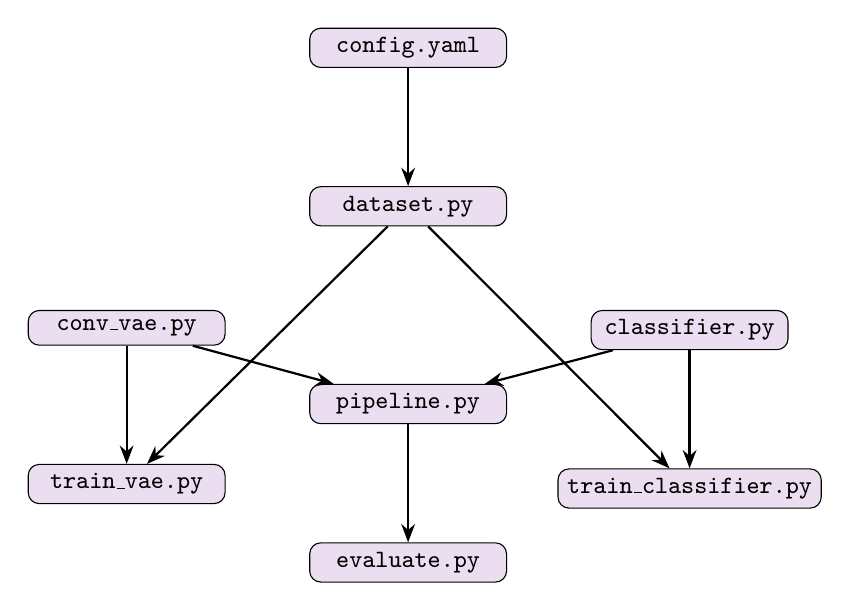
\begin{tikzpicture}[
    node distance=1.5cm,
    file/.style={draw, rounded corners, fill=filecolor!20, font=\ttfamily\small, minimum width=2.5cm},
    arrow/.style={-{Stealth}, thick}
]
    \node[file] (config) {config.yaml};
    \node[file, below=of config] (dataset) {dataset.py};
    \node[file, below left=of dataset] (vae) {conv\_vae.py};
    \node[file, below right=of dataset] (classifier) {classifier.py};
    \node[file, below=2cm of dataset] (pipeline) {pipeline.py};
    \node[file, below=of vae] (trainvae) {train\_vae.py};
    \node[file, below=of classifier] (traincls) {train\_classifier.py};
    \node[file, below=of pipeline] (evaluate) {evaluate.py};

    \draw[arrow] (config) -- (dataset);
    \draw[arrow] (dataset) -- (trainvae);
    \draw[arrow] (dataset) -- (traincls);
    \draw[arrow] (vae) -- (trainvae);
    \draw[arrow] (vae) -- (pipeline);
    \draw[arrow] (classifier) -- (traincls);
    \draw[arrow] (classifier) -- (pipeline);
    \draw[arrow] (pipeline) -- (evaluate);
\end{tikzpicture}
\end{center}

\end{document}
